%\documentclass[journal]{IEEEtran}
\documentclass{article}
\usepackage{amsmath}
\usepackage{listings}
\usepackage{graphicx}
\usepackage{multicol}
\usepackage{wrapfig}
\graphicspath{./imgs/}
\DeclareGraphicsExtensions{.pdf, .jpeg, .png}
\usepackage{geometry}
\geometry{a4paper, portrait, margin=1in}

\newcommand{\includecode}[2][c]{\lstinputlisting[caption=#2, escapechar=, language=#1]{#2}}
 
\hyphenation{op-tical net-works semi-conduc-tor}
\begin{document}

\title{Computational Physics Assignment 4}
\author{Austin~F.~Oltmanns}

\maketitle

% As a general rule, do not put math, special symbols or citations
% in the abstract or keywords.
\begin{abstract}
A 3D rendering system is developed and used to test simulation accuracy during large particle collisions. Accuracy
of conservation of energy is observed throughout the collision at different system temperatures.
\end{abstract} 

\section{Introduction}
%\IEEEPARstart{T}{his}
This assignment required students to expand upon code developed in class for simulating a non-ideal gas.
This particular assignment focused on setting up and using a 3D rendering system for 3 dimensional simulations.
Additionally, students were tasked with designing and performing their own experiment which utilized this system. 
The experiment outlined in this report is designed to determine the accuraccy of conservation of energy in 
the simulation code developed.

The experiment consisted of colliding 2 groups of particles and observing the temperature until the reaction reached
a steady state. The groups of particles were set to varying initial velocities (determining the energy/temperature of
the system) which caused them to collide. The results from these experiments are included and analyzed in this report.

For simplicity, real world units have been disregarded in an effort to keep the numbers used in the simulation from 
becoming very large or small (which can affect the stability of the simulation.
Each aspect of the simulation will be described in detail below and the code is attached as an appendix to this report.

\section{3D Rendering System}
\subsection{Description}
%ORDER
To effectivly visualize the simulation as it happens, it is necessary to be able to view it in 3 dimensions. For this
purpose, a rendering system was created which emulates a camera outside of the periodically bound box which contains
the simulation. This system takes the particles' coordinates in referance to the box which contains them and 
performs a coordinate transform to find those same particles coordinates in the coordinate 
system defined by the camera. Before projecting this image onto a plane,
the particles are sorted such that the ones furthest from the camera are drawn first so they do not
appear to be on top of the particles that are closer. After this step, the particles are finally projected 
onto a plane between the camera and the scene. The particles' shadows
on this plane are essentially the image that will be viewed. Additionally, the bounding box is 
rendered with a red dot origin and principle axes are highlighted in color.

To perform these operations, the GNU Scientific Library's wrapper for the Basic Linear Algebra Subprograms (BLAS).
This library and its C-language BLAS implementation (CBLAS) allow for matrix and vector math to take place in a 
C program. Additionally,
it would be possible to link the program against different implementations of CBLAS which could be optimized
for parralel computation. Meaning that this simulation is now scaleable and would perform well (at
 least in the rendering routine) on such a platform.

\subsection{Coordinate Transform}
\begin{figure}[!t]
\centering
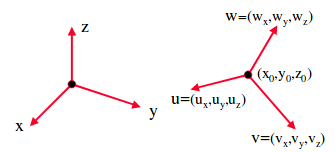
\includegraphics[width=3.5in]{./imgs/axes}
\caption{World and camera axes together. Camera axes have been defined with reference to the world axes.}
\label{fig:axes}
\end{figure}

The world coordinates are defined as points along 3 axes (shown in the Figs.~\ref{fig:partbefore}-\ref{fig:partafter}
 as the colored lines).
The camera can also be though of as having 3 different axes: one which extends in the direction it points, one which
points directly to its side and another which points directly up. Fig.~\ref{fig:axes} shows the two
sets of axes. The camera can also be rotated about each of these
axes independently in a pan/tilt/roll fashion. By defining the camera's axes as unit vectors from its position
in the direction of the axis, a transform matrix can be generated which transforms a point given in world coordinates
to the corresponding camera coordinates.

The first step is to determine the translation matrix which would translate the coordinates of a particle in world
coordinates to a set of coordinates which would be defined by the camera if it had no rotation relative to the world's
coordinate system. This matrix is denoted $T$ in Eqn.~\ref{eqn:trans}. 

\begin{equation}
T=
  \begin{bmatrix}
   1 & 0 & 0 & X_0 \\
   0 & 1 & 0 & Y_0 \\
   0 & 0 & 1 & Z_0 \\
   0 & 0 & 0 & 1
  \end{bmatrix}
  \label{eqn:trans}
\end{equation}


The second step is to find the rotation matrix 
which would transform the coordinates of a particle in world coordinates to that of the camera if it were located at 
the origen but rotated. This matrix is denoted $R$ in Eqn.~\ref{eqn:rot}.

\begin{equation}
R=
  \begin{bmatrix}
   U_x & V_x & W_x & 0 \\
   U_y & V_y & W_y & 0 \\
   U_z & V_z & W_z & 0 \\
   0 & 0 & 0 & 1
  \end{bmatrix}
  \label{eqn:rot}
\end{equation}

Finally, by combining these operations, the
final transformation matrix (denoted $M$ in Eqn.~\ref{eqn:total}) is obtained as the product of the two prior transforms
and points/particles described in world coordinates can be described in camera coordniates by applying Eqn.~\ref{eqn:doit}.

\begin{equation}
M = RT
\label{eqn:total}
\end{equation}

\begin{equation}
\begin{bmatrix}
  x' \\
  y' \\
  z' \\
  1
\end{bmatrix}
  = M
\begin{bmatrix}
  x \\
  y \\
  z \\
  1
\end{bmatrix}
\label{eqn:doit}
\end{equation}

To implement these equations, the following lines of code establish the cameras axis in world coordinates.
\begin{lstlisting}[language=c][frame=single]
//rotate by pan and tilt(rotation around Z/W)
gsl_vector_set_basis(renderman.camU, 0);
gsl_vector_set_basis(renderman.camV, 1);
gsl_vector_set_basis(renderman.camW, 2);
gsl_blas_drot(renderman.camU, renderman.camV, cos(mycam.roll), sin(mycam.roll));
gsl_blas_drot(renderman.camU, renderman.camW, cos(mycam.pan), sin(mycam.pan));
gsl_blas_drot(renderman.camV, renderman.camW, cos(mycam.tilt), sin(mycam.tilt));
\end{lstlisting}

The above section of code instantiates a set of axes for the camera as unit vectors along
 $\hat i$, $\hat j$ and $\hat k$. Then, the roll, pan and tilt of the camera is used to rotate pairs of 
axes around each respective axis for the rotation. After this, the next snippit of code uses this information
to populate the rotation and translation matrices.

\begin{lstlisting}[language=c][frame=single]
//form rotation and translation matrices
for (unsigned int i=0; i<3; i++)
{
  gsl_matrix_set(renderman.trans, i, 3, gsl_vector_get(mycam.pose, i));
  gsl_matrix_set(renderman.rot,   i, 0, gsl_vector_get(renderman.camU, i));
  gsl_matrix_set(renderman.rot,   i, 1, gsl_vector_get(renderman.camV, i));
  gsl_matrix_set(renderman.rot,   i, 2, gsl_vector_get(renderman.camW, i));
}
\end{lstlisting}

Then the total transformation matrix is calculated. The gsl\_blas\_dgemm function computes the product of two matrices
(in this case: renderman.rot and renderman.trans) and sums that product with a third matrix and stores the result
in that third matrix.

\begin{lstlisting}[language=c][frame=single]
//calculate total transformation matrix
gsl_blas_dgemm(CblasNoTrans, CblasNoTrans,  1, renderman.rot, renderman.trans,
               0, renderman.coordinateTransform);
\end{lstlisting}

Next, the coordinates can be transformed by another matrix multiplication. The positions of each particle have
been loaded into renderman.worldCoordHolder as an array of column vectors to form a 4xN matrix where N denotes the number of particles. Because
of how the sort method is constructed, this operation is done to return the transpose of the result by passing 
the 'CblasTrans' flag for each matrix which is being multiplied and inverting the order of multiplication. This
is a property of matrix multiplication and transposes.

\begin{lstlisting}[language=c][frame=single]
//perform total transformation
gsl_blas_dgemm(CblasTrans, CblasTrans, 1, renderman.worldCoordHolder, 
               renderman.coordinateTransform,  0, renderman.renderCoord);
\end{lstlisting}

\subsection{Sorting by Distance}
After the coordinates are transformed but before they are projected onto the imaging plane, they must be sorted by
distance from the camera so the furthest particles are drawn first so they appear behind the particles that are closer.

This is accomplished via the C standard library function qsort. Each particle's position in camera coordinates 
has been recorded in the renderman.renderCoord matrix. Because the color information of each particle must persist, it is 
necessary to keep track of each particles color before it is sorted. Thankfully, the matrix math from above 
has left a matrix which has an auxillary 1 below each coordinate. At this point, it will no longer be used
to perform matrix math, so it can be replaced with color information before the sort takes place.

The following code demonstrates the procedure:

\begin{lstlisting}[language=c][frame=single]
int compare(const void *x1,const void *x2){
  if (((double *) x1)[2]< ((double *)x2)[2]) return 1;
  else return -1;
}

...

//sort rendercoord by camera distance
//assign color
for (unsigned int i=0; i<NUM_PARTICLES; i++)
{
  gsl_matrix_set(renderman.renderCoord, i, 3, i%3 +2);
}
//sort by depth
qsort(gsl_matrix_ptr(renderman.renderCoord,0,0), NUM_PARTICLES, 
                     4*sizeof(double), &compare);
\end{lstlisting}

\subsection{Projection onto a Plane}
Now that the points can be described in camera coordinates, they must be projected onto a 2D screen. This part is 
somewhat simpler than the coordinate transform because it simply uses similar triangles for the calculation. 
A point in camera coordinates will be shown on the plane as having its distance from the origin of the plane
(defined as the point orthogonal to the plane and through the camera) scaled by the distance from the plane
to the camera divided by the distance of the particle to the camera. The distance from the plane to the camera
is the focal length of the camera (mycam.zoom in the below code). This method is known as a perspective projection. 
Once the points have been projected onto this plane, it is trivial to scale this plane to the rendering area 
(a window on a computer monitor). The following snippit of code demonstrates this procedure:

\begin{lstlisting}[language=c][frame=single]
//display particles
for (unsigned int i=0; i<NUM_PARTICLES; i++)
{
  int xdraw = mycam.zoom * gsl_matrix_get(renderman.renderCoord, i, 0) 
              / gsl_matrix_get(renderman.renderCoord, i, 2) + (double)xdim/2.0;
  int ydraw = mycam.zoom * gsl_matrix_get(renderman.renderCoord, i, 1) 
              / gsl_matrix_get(renderman.renderCoord, i, 2) + (double)ydim/2.0;
  myfilledcircle((int) gsl_matrix_get(renderman.renderCoord, i, 3), xdraw, ydraw, 3);
}
\end{lstlisting}


\subsection{Bounding Box}
Using the same technique that was used to project the points onto the screen, corner points from the experiments
periodically bound box are transformed to points in the rendering window and lines are drawn between them, displaying
the outline of the bounding box. For brevity, its implementation is not shown here. Instead, Fig.~\ref{fig:partbefore}
shows the rendered image of particles initialized and ready to collide.

\begin{figure}[b!]
\centering
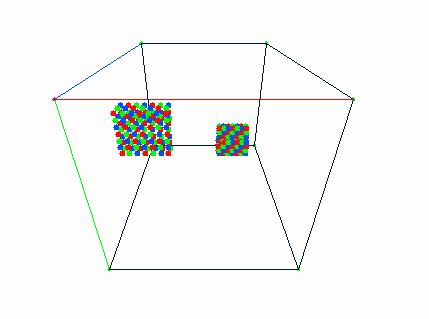
\includegraphics[width=3.0in]{./imgs/particlesbefore}
\caption{Particles initilaized before being collided.}
\label{fig:partbefore}
\end{figure}

\section{Conservation Experiment}
\subsection{Description}
In order to determine how well energy is conserved, two packets of 120 particles each were sent at each other at 8
different speeds corresponding to 8 different initial system temperatures. If energy is conserved well in the 
simulation, the temperature should remain constant throughout the reaction. Otherwise, the temperature will
change throughout the reaction.

\subsection{Results}
\begin{multicols}{2}

%figures of before during and after

\begin{wrapfigure}{l}{.8\linewidth}
\centering
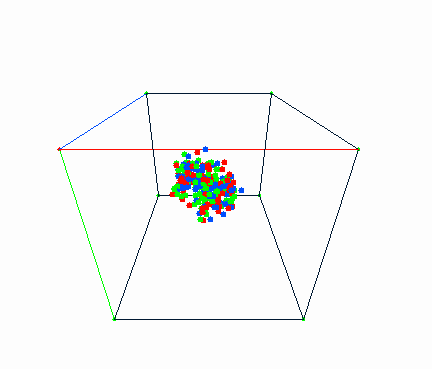
\includegraphics[width=\linewidth]{./imgs/particlesduring}
\caption{Particles colliding.}
\label{fig:partduring}
\end{wrapfigure}

\begin{wrapfigure}{l}{.8\linewidth}
\centering
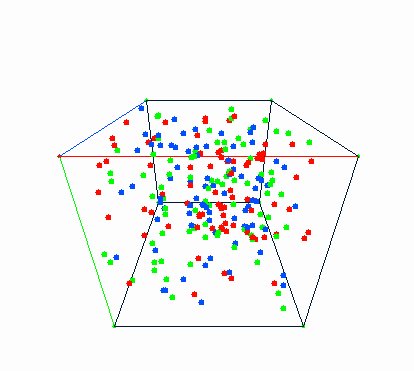
\includegraphics[width=\linewidth]{./imgs/particlesafter}
\caption{Particles some time after the collision.}
\label{fig:partafter}
\end{wrapfigure}


\begin{wrapfigure}{l}{.8\linewidth}
\centering
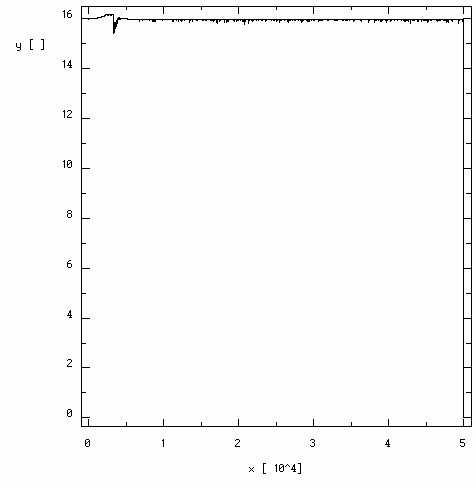
\includegraphics[width=\linewidth]{./imgs/temp16_0}
\caption{Temperature vs Time in seconds for $T_0$=16}
\label{fig:temp1}
\end{wrapfigure}

\begin{wrapfigure}{l}{.8\linewidth}
\centering
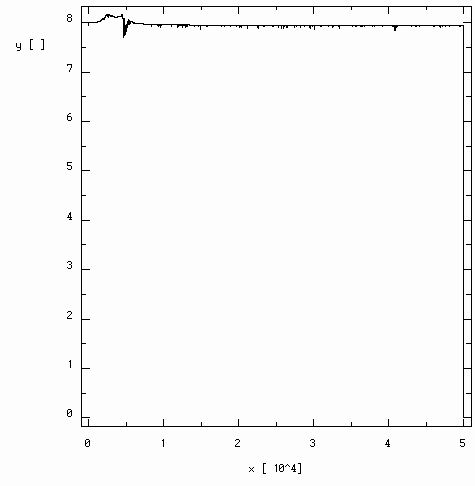
\includegraphics[width=\linewidth]{./imgs/temp8_0}
\caption{Temperature vs Time in seconds for $T_0$=8}
\label{fig:temp2}
\end{wrapfigure}

\begin{wrapfigure}{l}{.8\linewidth}
\centering
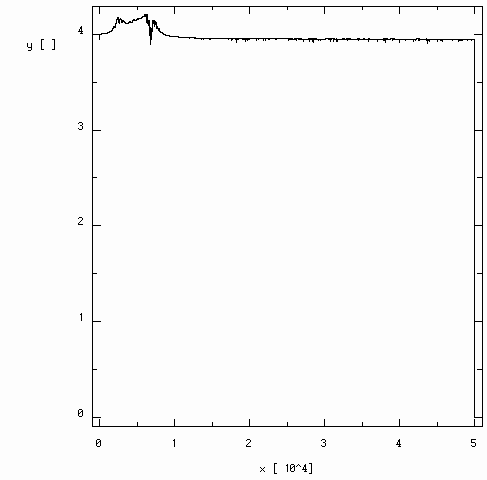
\includegraphics[width=\linewidth]{./imgs/temp4_0}
\caption{Temperature vs Time in seconds for $T_0$=4}
\label{fig:temp3}
\end{wrapfigure}

\begin{wrapfigure}{l}{.8\linewidth}
\centering
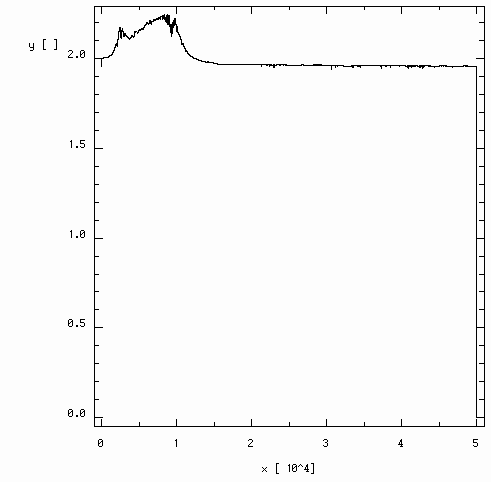
\includegraphics[width=\linewidth]{./imgs/temp2_0}
\caption{Temperature vs Time in seconds for $T_0$=2}
\label{fig:temp4}
\end{wrapfigure}

\begin{wrapfigure}{l}{.8\linewidth}
\centering
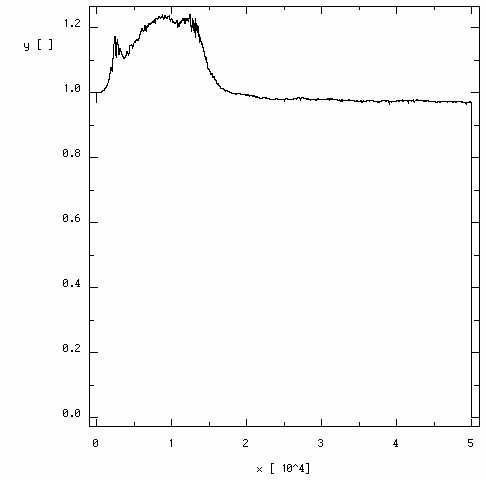
\includegraphics[width=\linewidth]{./imgs/temp1_0}
\caption{Temperature vs Time in seconds for $T_0$=1}
\label{fig:temp5}
\end{wrapfigure}

\begin{wrapfigure}{l}{.8\linewidth}
\centering
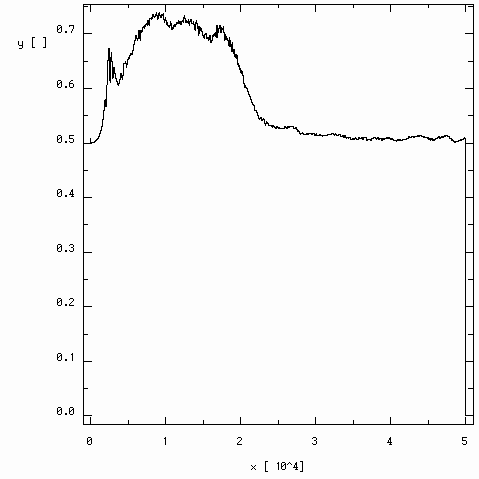
\includegraphics[width=\linewidth]{./imgs/temp_5}
\caption{Temperature vs Time in seconds for $T_0$=0.5}
\label{fig:temp6}
\end{wrapfigure}

\begin{wrapfigure}{l}{.8\linewidth}
\centering
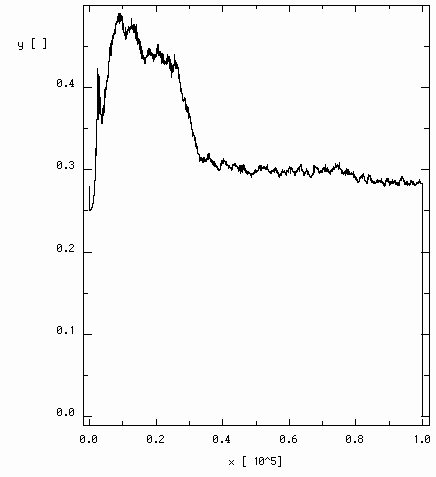
\includegraphics[width=\linewidth]{./imgs/temp_25}
\caption{Temperature vs Time in seconds for $T_0$=0.25}
\label{fig:temp7}
\end{wrapfigure}

\end{multicols}

\begin{figure}[h!]
\centering
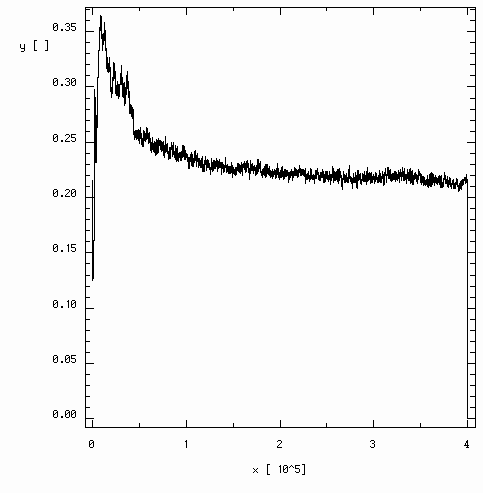
\includegraphics[width=2.5in]{./imgs/temp_125longer}
\caption{Temperature vs Time in 10's of seconds for $T_0$=0.125}
\label{fig:temp8}
\end{figure}

%figures of graphs

\subsection{Analysis}
It can be seen clearly that energy is not conserved well, especially in lower temperature situations. However, in 
higher temperature situations energy is conserved better. In the lowest temperature test 
(seen in Fig.~\ref{fig:temp8}), the system does not appear
to be returning to the initial conditions. Even if it is, it is taking far to long to be useful if other events
had to take place in the situation. On the other end of the spectrum, the high temperature simulations return to 
the initial temperature as the system settles.


\section{Conclusion}
Obviously there are approximations which take place in a simulation. The question a simulator must ask is how
much approximation is acceptable and how much error can be allowed. The data from these experiments show that this
module should most likely not be used for low temperature collisions of groups of gas particles. However, at higher
temperatures the resuslts could be acceptable depending on application.

Additionally, the 3D rendering system outlined in this report is very modular and could be extended easily to 
do things like having the camera follow a path or track certain elements throughout the simulation.

The code used to complete this assignment is attached as an appendix to this document.

\section{References}
http://www.math.tau.ac.il/~dcor/Graphics/cg-slides/geom3d.pdf

http://www.cse.psu.edu/~rtc12/CSE486/lecture12.pdf

\newpage
\onecolumn
\section{Appendix}
\lstinputlisting[language=c]{../src/program.c}
\end{document}